% Date of the last edit of these instructions
\def \lastedit{June 20, 2019}

\documentclass[paper=a4,parskip=full+]{scrartcl}
\usepackage[utf8]{inputenc}
\usepackage{titletoc}
\usepackage[margin=1in]{geometry}
\usepackage{float}
\usepackage{parskip}
\usepackage{graphicx}
\graphicspath{ {Images/} }

\title{OreSat Live HGS Assembly}
\date{Last Edited: \lastedit}

\begin{document}

\maketitle
\tableofcontents

\section{Introduction}
This document provides instructions for assembling the Handheld Ground Station with a kit.
\section{Overview of Required Materials}
\subsection{The Kit}
The kit comes with the following items:
\begin{itemize}
    \item Back-plane Circuit board
    \item 75mm U.FL to U.FL Coax Cable
    \item 63" of 20-gauge Magnet Wire
    \item Raspberry Pi Zero W
    \item WF-NP9202 Atheros Wireless Module
    \item Micro USB to Wireless Module Connector Cable
    \item 6" USB A to Micro B Cable
    \item 5000mAh Battery with USB
    \item $1/4$"-20 nut for tripod mounting
    \item 1.5" Hook-and-loop Velcro (adhesive-backed)
    \item Plastic Components
    \begin{itemize}
        \item Handle
        \item Screw Block
        \item Phone Holder Base
        \item Phone Holder Slide
        \item Battery Holder
        \item Antenna Sections x4
        \item Antenna Top Cap
        \item Antenna Bottom Cap
    \end{itemize}
\end{itemize}

\subsubsection{Board Check}
Please check that the backplane board comes with both a U.FL connector and a 8.2pF capacitor already soldered on to the board. 
% PICTURE HERE of microstrip, U.FL connector and pF cap soldered on board

\subsection{Parts Not Provided}
The parts below are not a part of the kit but still needed to assemble the HGS.\\
\textbf{*Note: You DO NOT have to use the sources specified in these tables.}
\begin{table}[H]
    \footnotesize
    \begin{tabular}{|l|l|l|l|l|}
        \hline
        Quantity & Description & Source & Manufacturer & Part Number\\
        \hline
        \hline
        4 & \#8-32 x 1" Screws and Hex Nuts & Home Depot & Everbilt & 460 626 \\
        \hline
        4 & \#8-32 x 1.5" Screws and Hex Nuts & Home Depot & Everbilt & 461 400 \\
        \hline
        7 & \#2-56 x 3/8 Nylon Screw & Frys & Waldom & FN-816-0025P \\
        \hline
        7 & \#2-56 Nylon Lock Nut & Frys & Waldom & FN-502-0025P \\
        \hline
        7 & \#2-56 Nylon Hex Nut & Frys & Waldom & FN-853-0025P \\
        \hline
        & Foam Tape - Camper Seal 3/16" x 1 1/4" & & & \\
        \hline
        1 & Rubber Band of your choosing & & & \\
        \hline
        
    \end{tabular}
    \label{tab:my_label}
\end{table}

\noindent The following are optional items for easy clamping while gluing or assembly without glue:

\begin{table}[H]
    \footnotesize
    \begin{tabular}{|l|l|l|l|l|}
    \hline
    Quantity & Description & Source & Manufacturer & Part Number\\
    \hline
    \hline
    1 & \#8-32 x 18 in threaded rod & Home Depot & & \\
    \hline 
    1 & 1/8in x 1 in fender washer & Home Depot & Everbilt & 210 364 \\
    \hline 
    1 & \#8-32 wing nuts & Home Depot & Everbilt & 934 917 \\
    \hline 
    \end{tabular}
\end{table}

\noindent You can substitute \#2-56 for M2 and \#8-32 for M4.

\newpage
\section{Assembly Instructions}
Do these things!
\subsection{Overview}
The core of the HGS is the circuit board/antenna back-plane, all the other components are in some way attached to it. The main electrical component we are concerned with is the wire wrapping the main antenna. It is soldered on the board to an impedance matching strip, strung through a hole in the board, wrapped around the antenna, and epoxied under a cap at the tip. For this reason the initial steps must be done in a particular order to ensure ease of assembly.

\subsection{Assemble antenna segments (no caps)}
First we will epoxy together the four antenna segments, without the end-caps.

(A threaded rod may be used to replace the epoxy. If using a threaded rod, ignore the sections about epoxying things, and in the section about winding the wire, use the threaded rod to hold everything together other than the cap, and clamp down the rod once the wire is wound.)

(For each section using epoxy, follow the manufacturers instructions for mixing, usage, and cure times. Make sure not to mix so much at one time that it starts to set before you have time to apply it all!)

Mix together a small batch of epoxy and apply it liberally to the end of one of the antenna segments, then insert the peg of another segment and apply pressure until the epoxy has set. Repeat until all four sections are connected as one antenna.

Make sure to wipe off any excess epoxy after clamping, to avoid filling the grooves.

\begin{figure}[H]
    \centering
    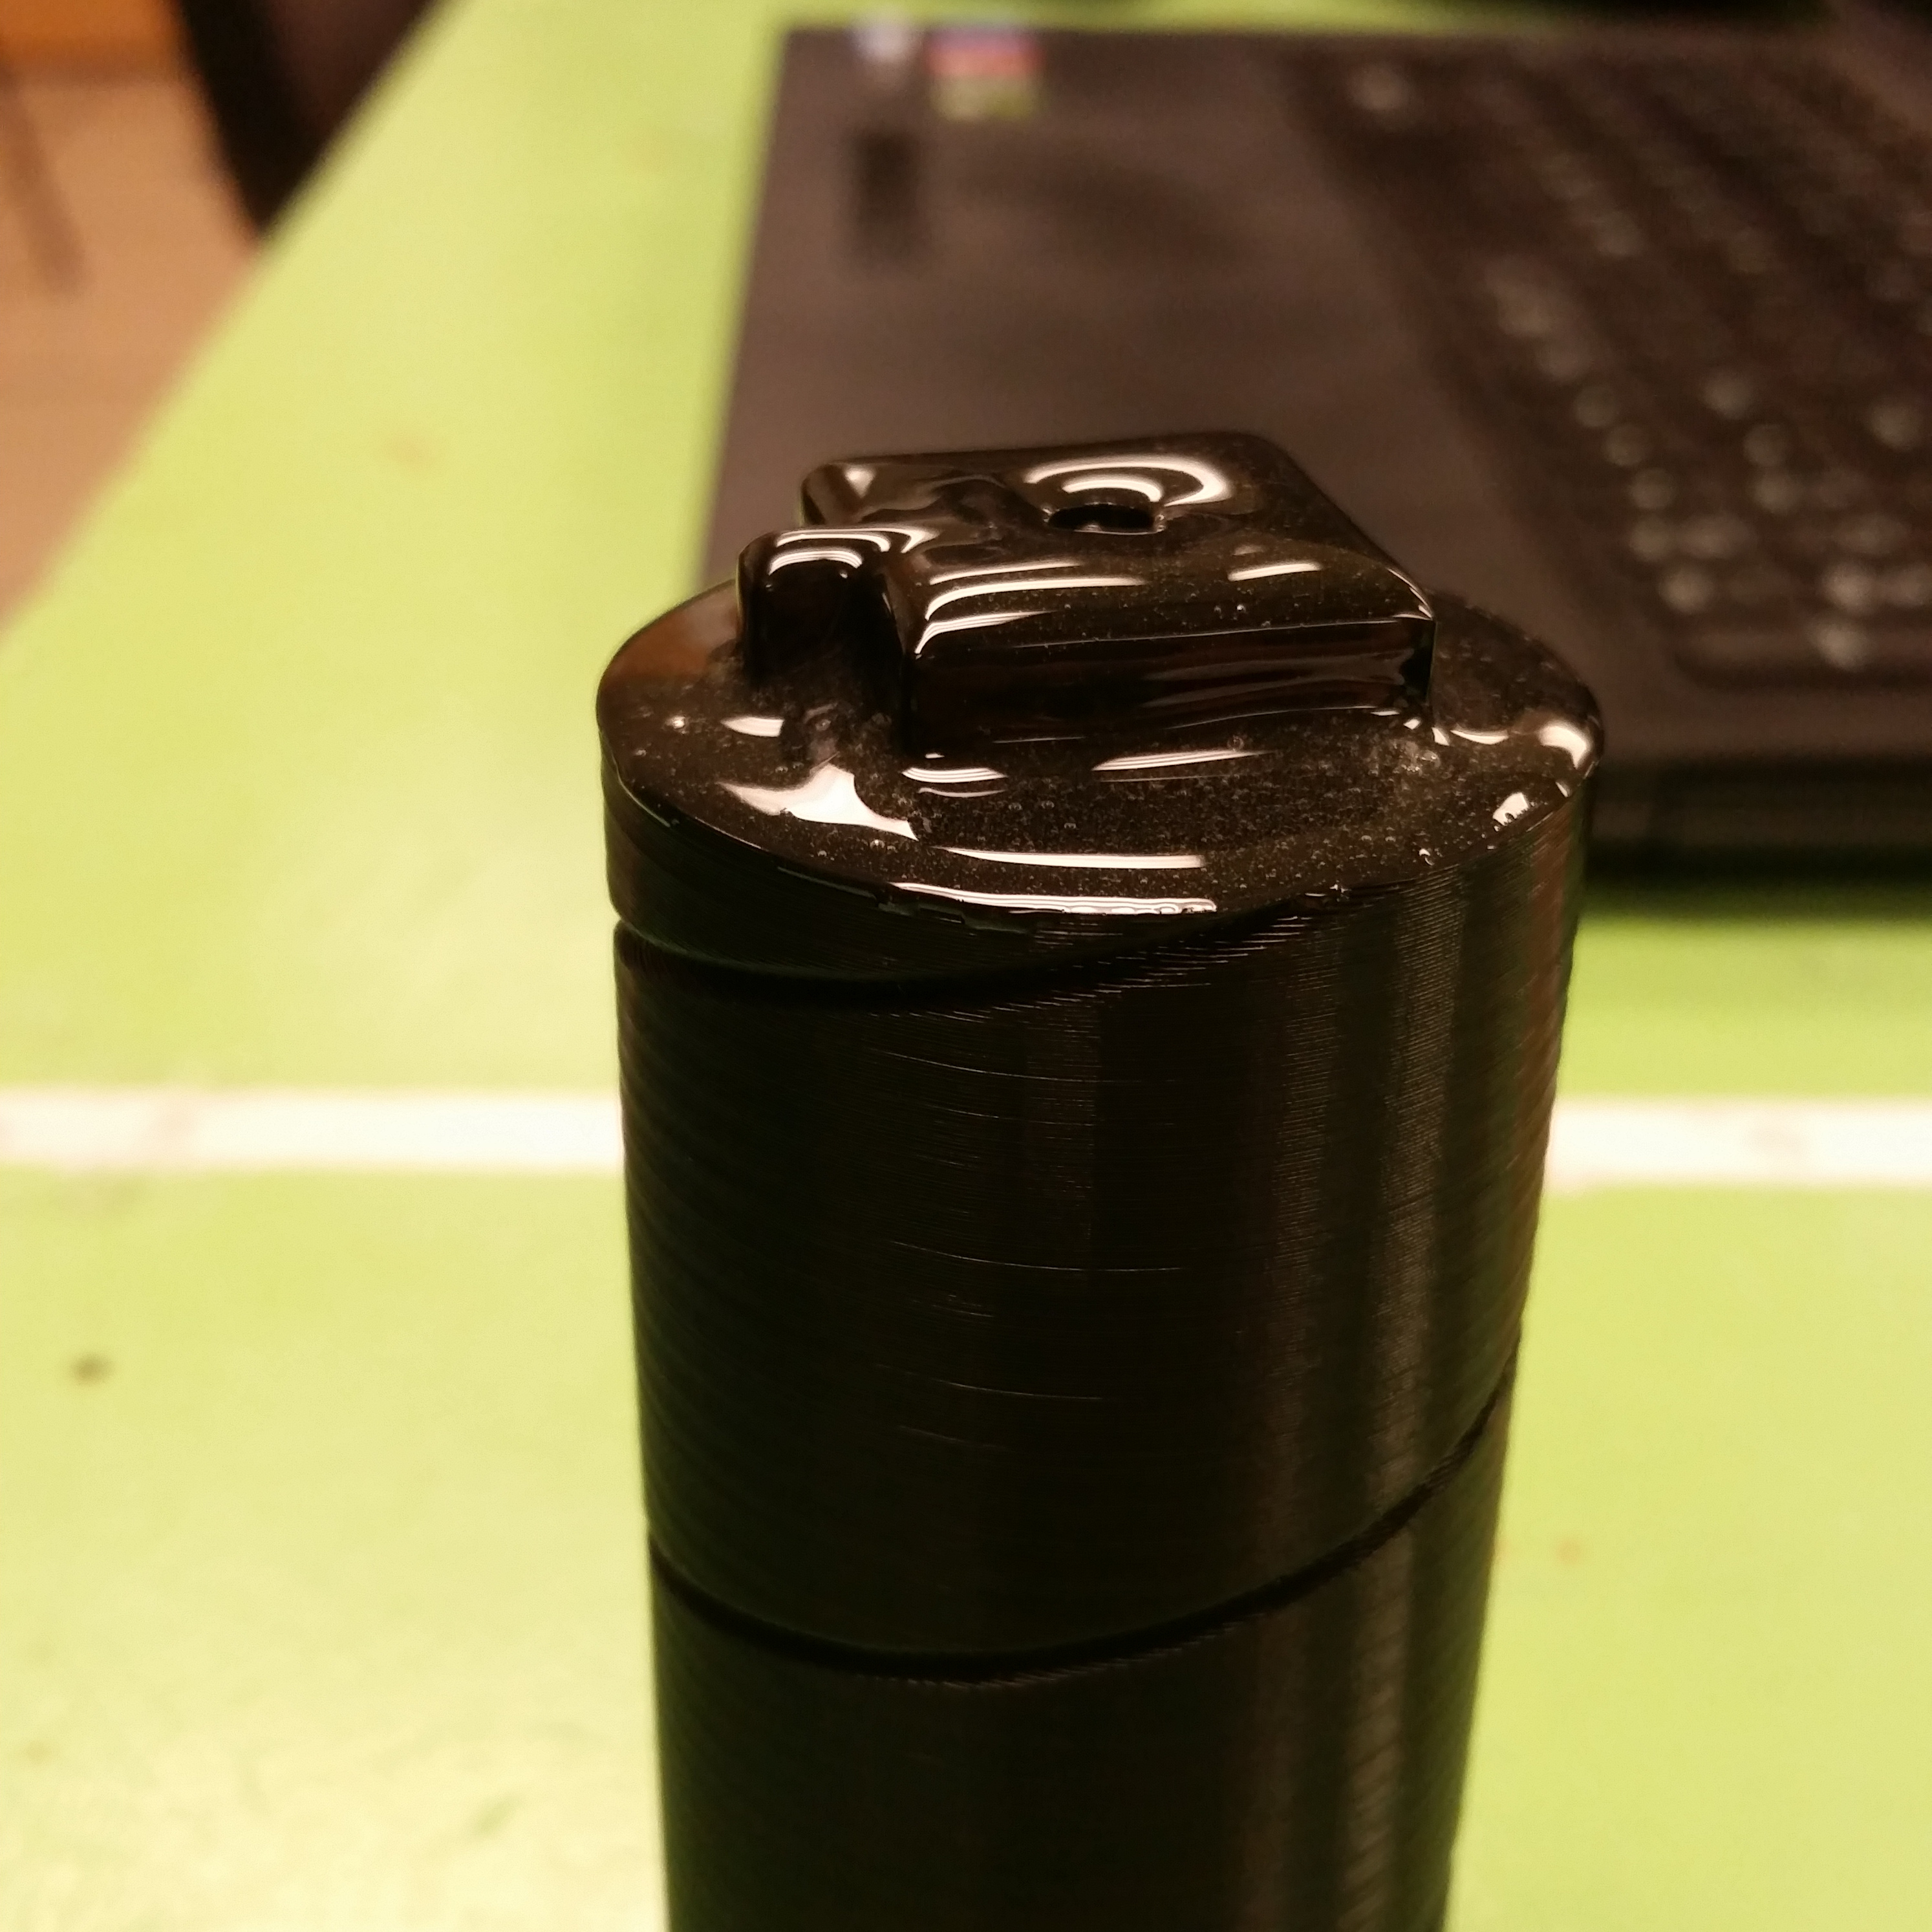
\includegraphics[width=0.45\textwidth]{Epoxy.jpg} 
    %Photo of epoxy covered antenna cap.
\end{figure}

%PHOTO OF ASSEMBLED ANTENNA

\subsection{Solder antenna wire onto micro-strip pad}
Solder one end of your wire to the bare end of the micro-strip, holding the wire perpendicular to the micro-strip. Snip off any excess wire.

Stick the rest of the wire through the nearby hole to the other side of the board for winding later.

%PHOTO HERE OF SOLDERED BOARD CLOSEUP

\subsection{Epoxy antenna to circuit board}
(Skip this section if using a threaded rod.)

Apply epoxy liberally to the peg end of the antenna, and the hollow end of the antenna clamp, push the antenna through the board, leaving the antenna on the side opposite the micro-strip, put the clamp piece on the end of the peg, sandwiching the circuit board, and clamp until the epoxy is set.

%PHOTO OF BOARD WITH ANTENNA

\subsection{Wind antenna with wire}
Take the antenna, and pulling tight against the soldered end, wrap the wire around the antenna rod, following the groove.

When the wire reaches the top, push it into the groove at the top around the tie-off peg and pull tight. (See photo.)

\begin{figure}[H]
    \centering
    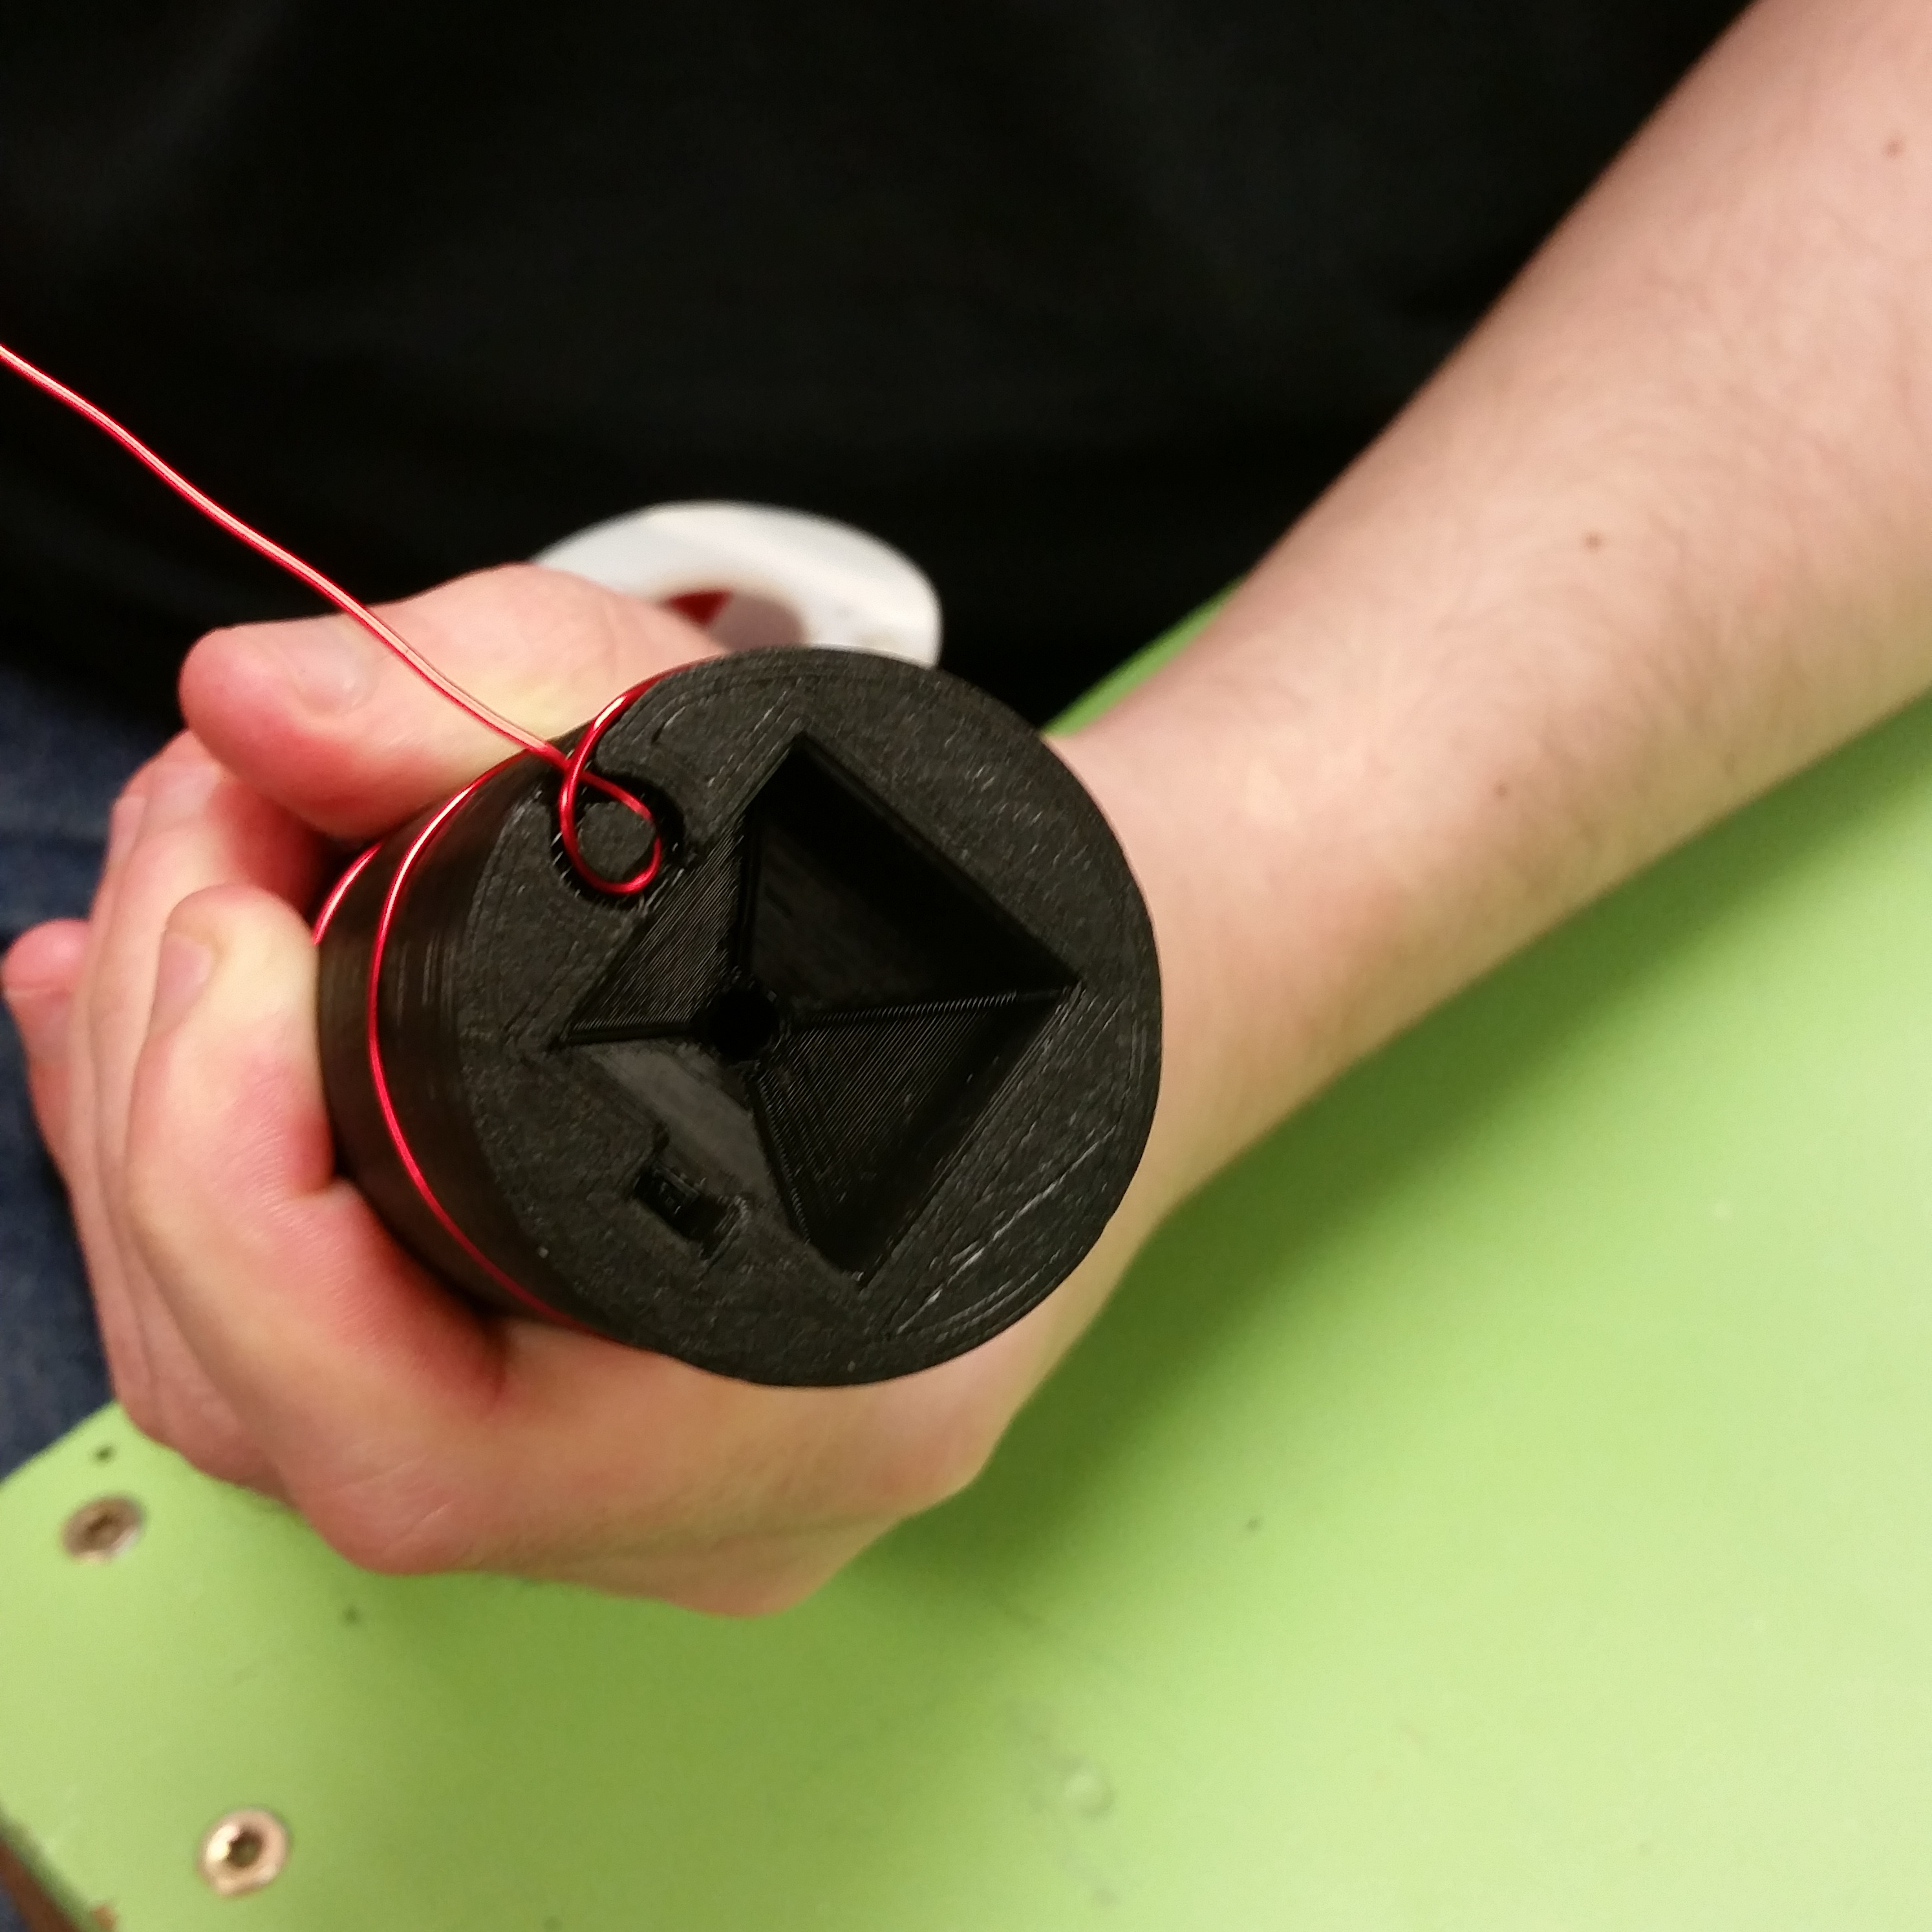
\includegraphics[width=0.6\textwidth]{Antenna_Wire_Tieoff.jpg} %Photo of wire tie-off.
\end{figure}

\noindent With wire tightly wrapped, apply epoxy liberally to the end of the antenna cap piece, and clamp down onto the tip of the antenna until the epoxy is cured to hold down the antenna.

Snip off any excess wire.

%PHOTO OF FULLY ASSEMBLED ANTENNA

\subsection{Attach plastic and electronic components}
Now that the antenna is attached, next we'll add the electrical components, and other 3D printed parts.

Start by adding the electronics: The Raspberry Pi, and the Atheros Wifi Module. Use the \#2-56 nuts and bolts, along with nylon standoffs to attach them to the side of the board opposite the antenna in the locations marked on the board. (In the future this will be referred to as the "back" of the board.)

%PHOTO OF BOARD WITH ELECTRICAL COMPONENTS INSTALLED

Plug the U.FL connector into the Atheros and the end of the micro-strip.

%PHOTO OF ENDS OF U.FL PLUGGED IN

Next with the \#8-32 x 1.5" screws, install the Handle, and on top of it the Battery Holder, using the square Handle Clamp piece to sandwich the board. The Handle itself and the Battery Holder go on the back of the board, with the Clamp piece on the front.

Install the Phone Holder Base above the handle, on the back of the board, with the open slot facing up using the \#8-32 x 1" screws.

%PHOTO OF HANDLE WITH BATTERY HOLDER INSTALLED

Install the sticky-backed foam into the faces the top and bottom of the Phone Holders to grip the phone, then slide the Phone Holder Top into the slot.

Wrap a rubber band between the top and bottom phone holder pieces to hold them together and hold the phone when in use.

Apply the Velcro to the top of the Battery Holder, and the Battery itself, as shown in picture.

\begin{figure}[H]
    \centering
    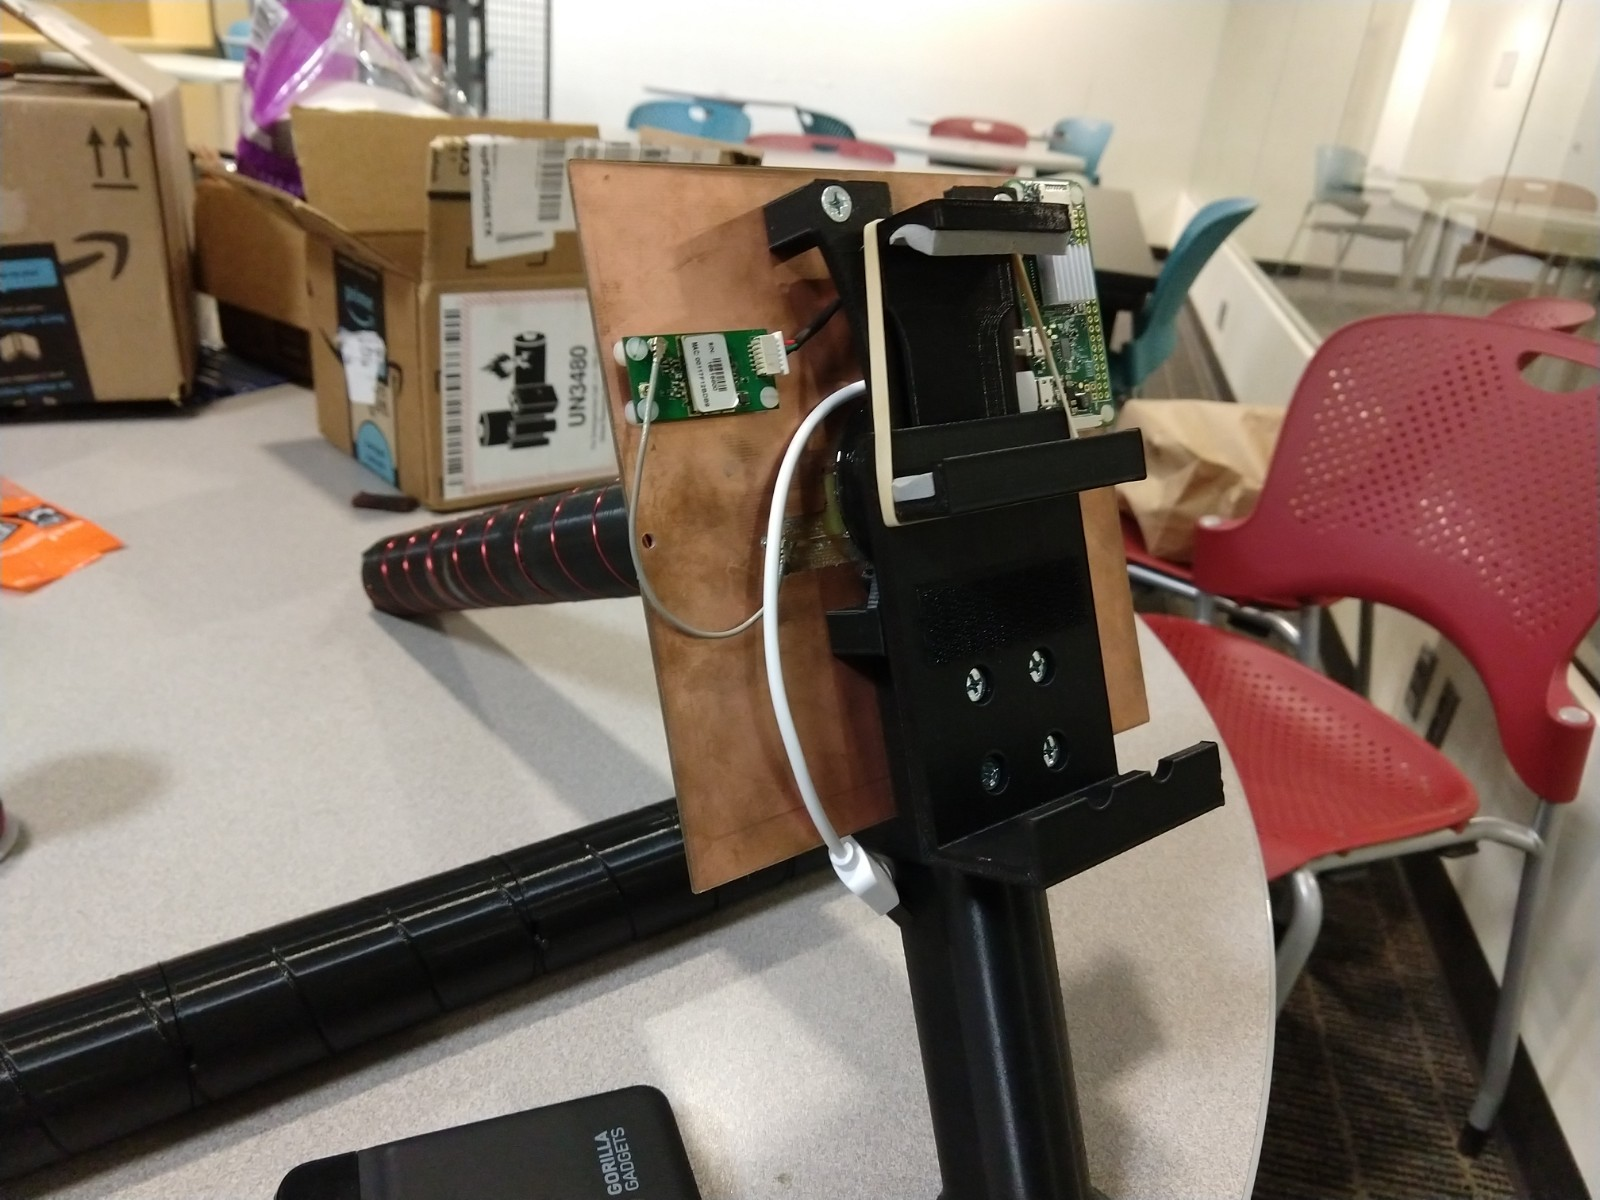
\includegraphics[width=0.45\textwidth]{Rubber_Band_and_Velcro.jpg} %Photo of phone and battery holders with Velcro and rubber bands installed.
    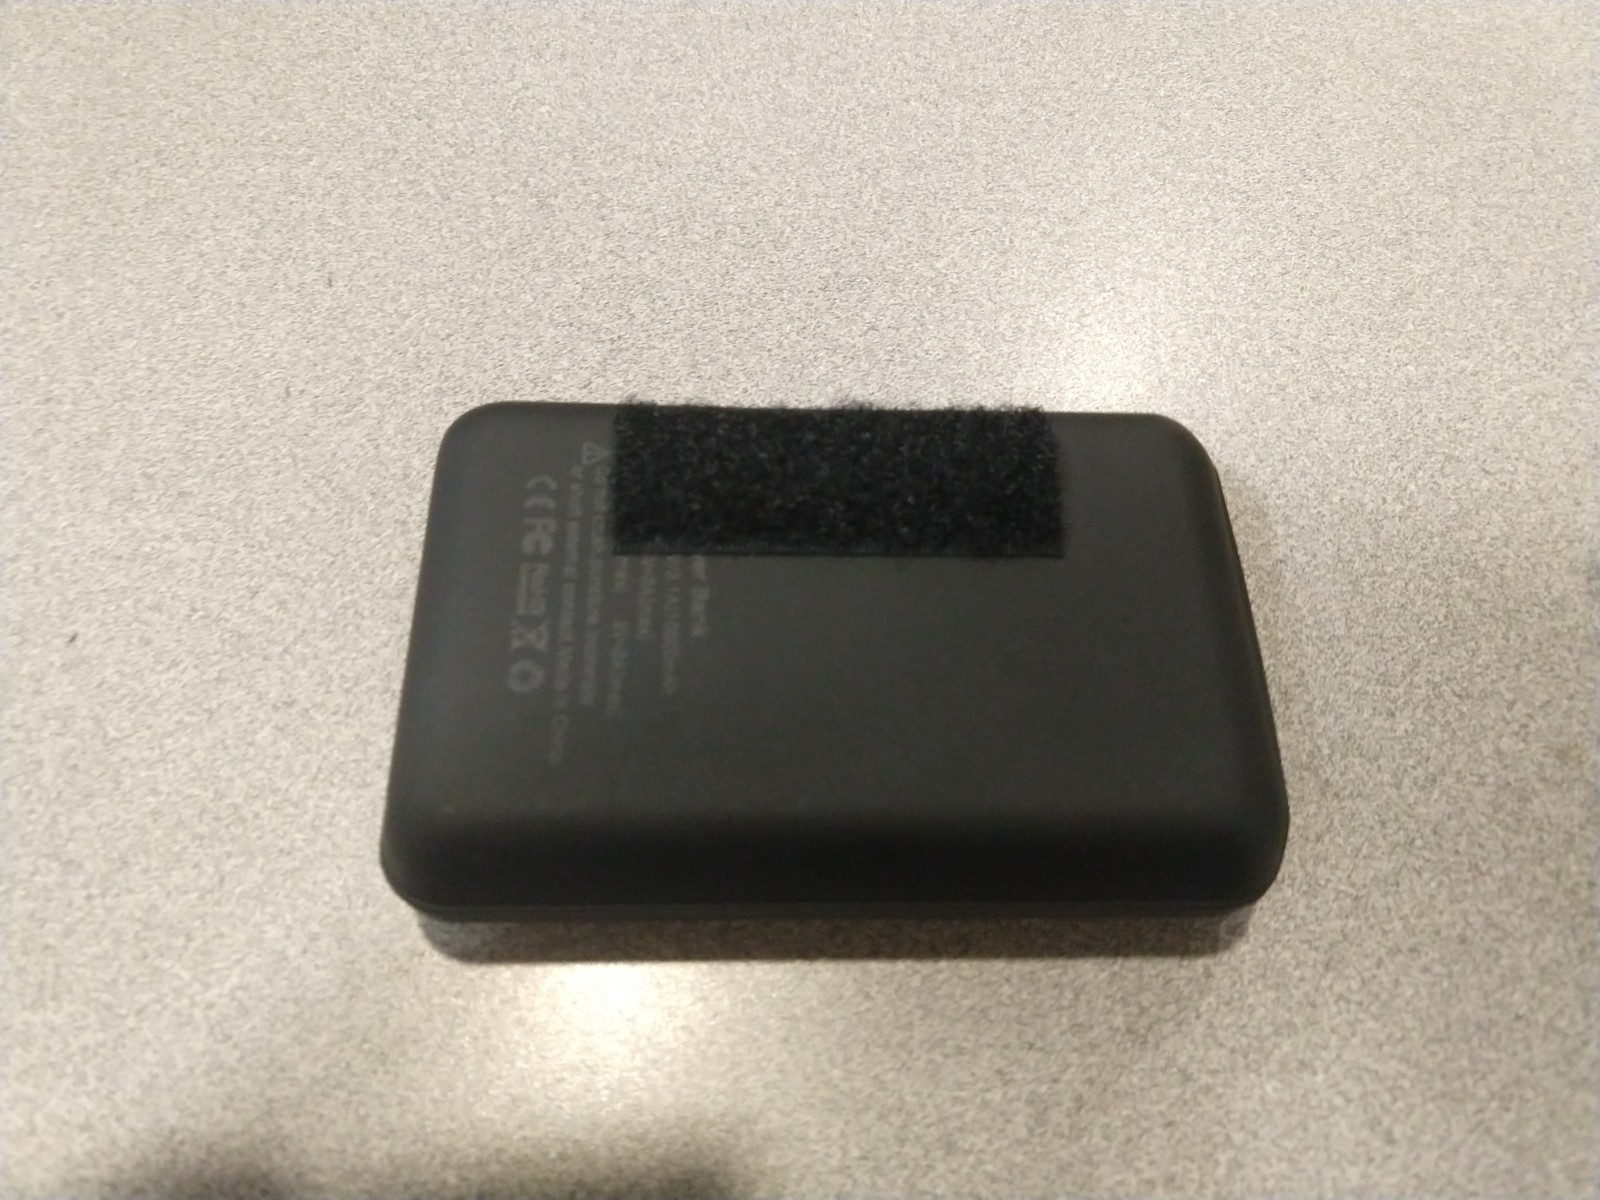
\includegraphics[width=0.45\textwidth]{Battery_Velcro.jpg} %Photo battery with Velcro installed.
\end{figure}

Then place the battery into the holder and rock forward to install. (Do not plug into the Raspberry Pi until ready to test!)

\begin{figure}[H]
    \centering
    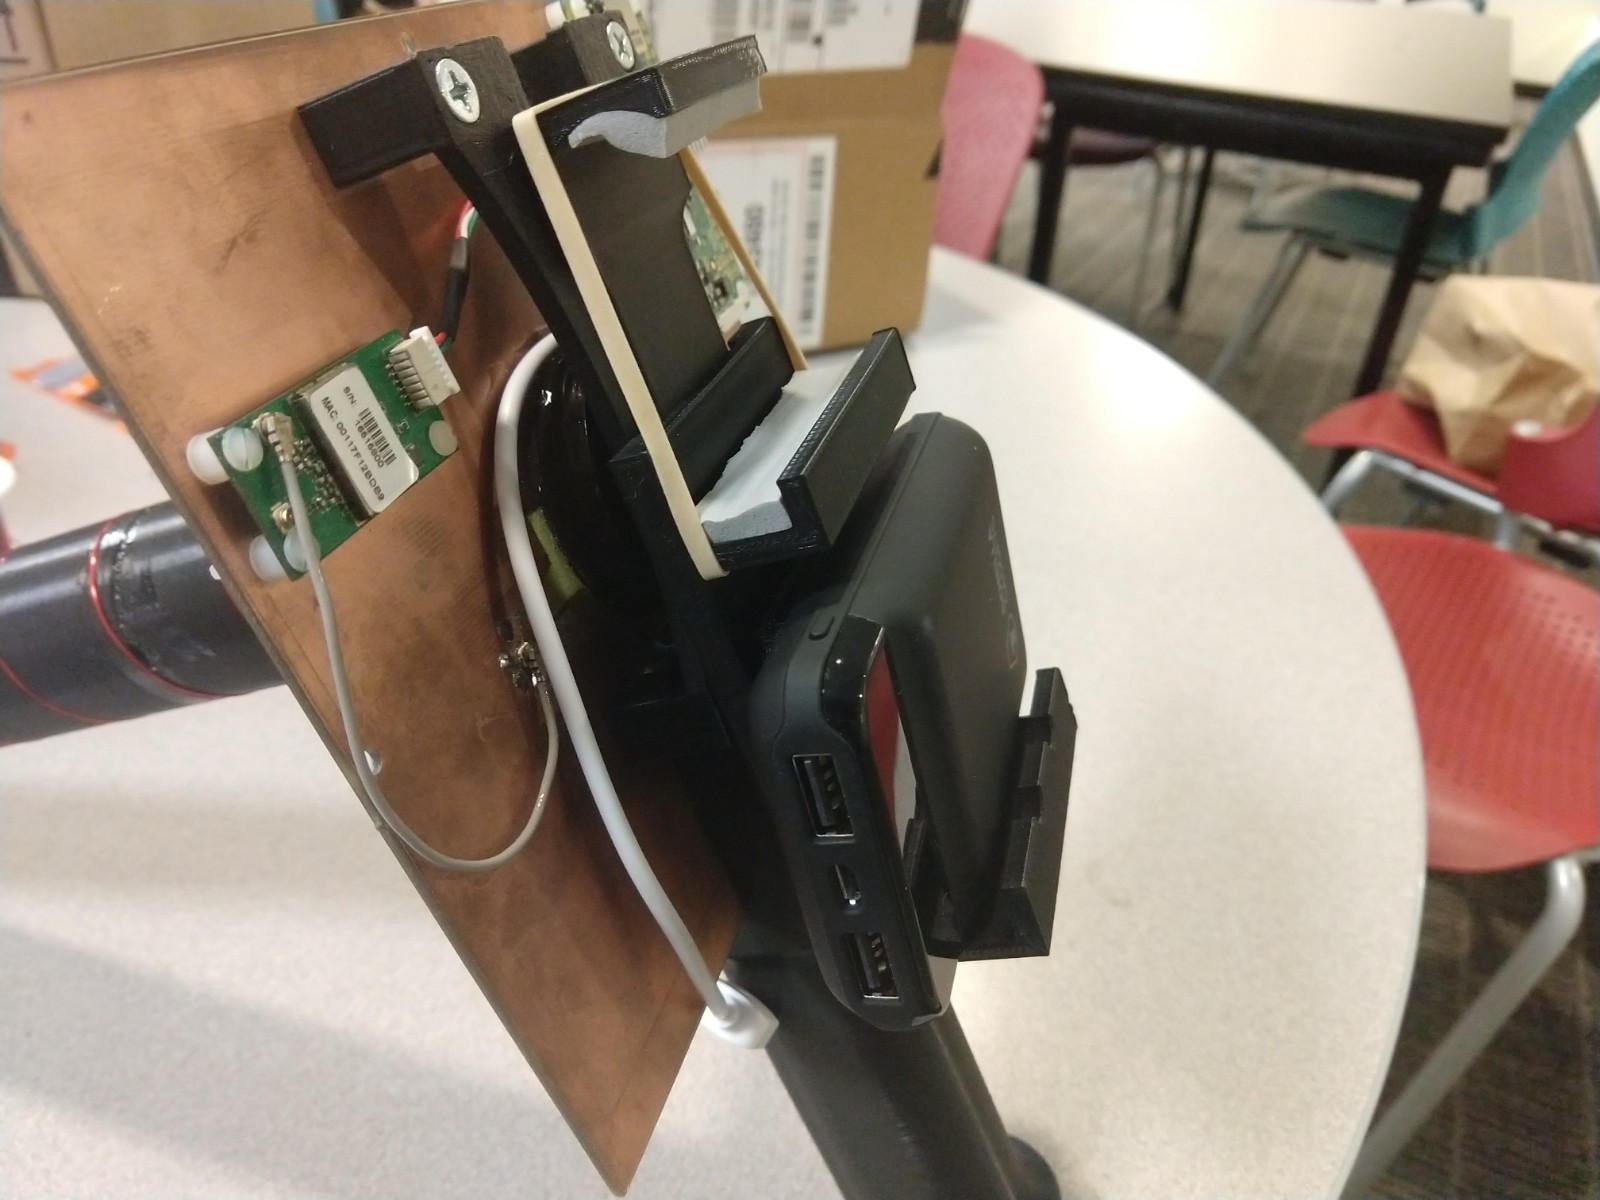
\includegraphics[width=0.6\textwidth]{Battery_Inserted.jpg} %Photo of Battery Holder with Battery installed.
\end{figure}

For usage, simply lift the top sliding section of the phone holder, and insert your phone, try to keep the power button clear of the clamp!

\begin{figure}[H]
    \centering
    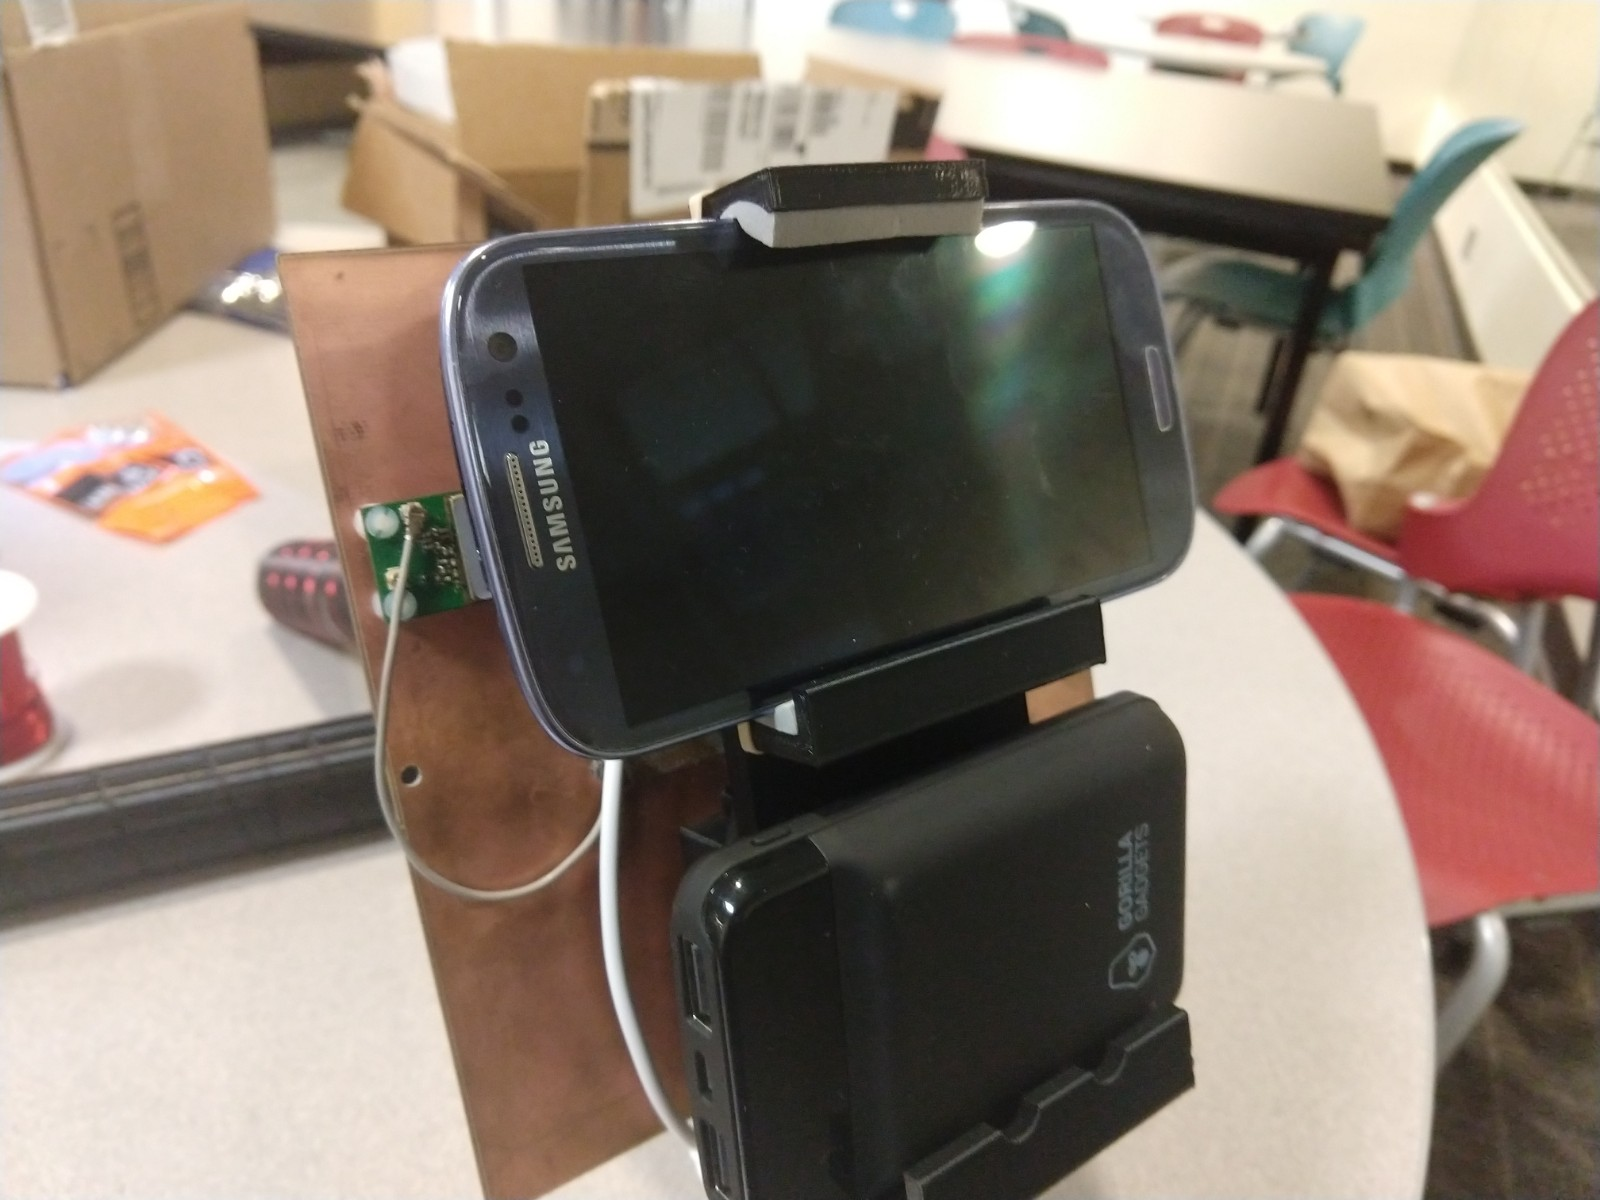
\includegraphics[width=0.6\textwidth]{Phone_Inserted.jpg} %Photo of Full assembly with phone inserted.
\end{figure}

Congratulations, assembly is complete! Make sure to test the full assembly to make sure the electrical connections are good, and you can connect to the access point and view the webpage.

\end{document}
